%!TEX root = ../../prace.tex

\chapter{Úvod}

V době vzniku této práce jsou velice populární hry s~otevřeným světem. Lákají hráče na obsáhlost světa a~možnost nelineárního řešení problémů a~herních úkolů. Her s~otevřeným světem najdeme nepřeberné množství v~různých herních žánrech. My se zaměříme na podmnožinu her, které kromě otevřeného světa nabízí také možnosti budování struktur a~vyžadují od hráče netriviální styl hraní, který mu umožňuje ve hře přežít. V herním průmyslu se tyto hry často označují jako \textit{sanboxové}, \textit{s budováním}, \textit{s průzkumem prostředí}, \textit{o přežití}. Autor této práce má tento typ her v~oblibě a~rád by touto prací představil svoji vizi dalšího možného rozvoje her tohoto žánru. Cílem práce by měla být implementace nového herního principu stavění, které současné herní tituly nenabízí.

\section{Charakteristika her}
V práci se budeme zabývat několika různými hrami, které však mají několik společných vlastností. Jedním ze základních konceptů je využívání herních bloků. Dalším význačným prvkem je způsob integrace herních bloků do herního prostření. Některé hry jsou celé tvořeny bloky, jiné se snaží dosáhnout vyššího stupně realismu ve hře a~bloky využívají pouze pro konstrukci různých herních objektů. Důležitým tématem této práce tedy bude rozbor systému bloků a~práce s~nimi a~popis hráčských problémů způsobených danými koncepty. V další části práce pak navrhneme a~implementujeme vlastní řešení.




\subsection{Hry kompletně blokové}
Začněme hrami, které využívají bloků jako základního elementu celé hry. Bloky zde tvoří doslova celý svět. Mezi nejpopulárnější a~širokou veřejností nejznámější bychom měli zařadit hru \MC{}. Na obrázku z této hry \ref{fig:intro_mc} si můžeme všimnout několika zásadních faktů. Vidíme zde kostičkované listí stromů (1) či hrad na skále (2), který byl postaven z~kostiček. Taktéž slunce, měsíc a~mraky (3) jsou stylizovány do kostiček. Výrazně je kostičkovaný styl vidět na nehratelných postavách (\textit{non-playable character} -- \NPC{}) -- na obrázku ovce (4), krávy a~prasata. Stejným způsobem je pak zpracován i~hráčův charakter (5), tedy postava, kterou hráč přímo ovládá.



\begin{figure}[!ht]\centering
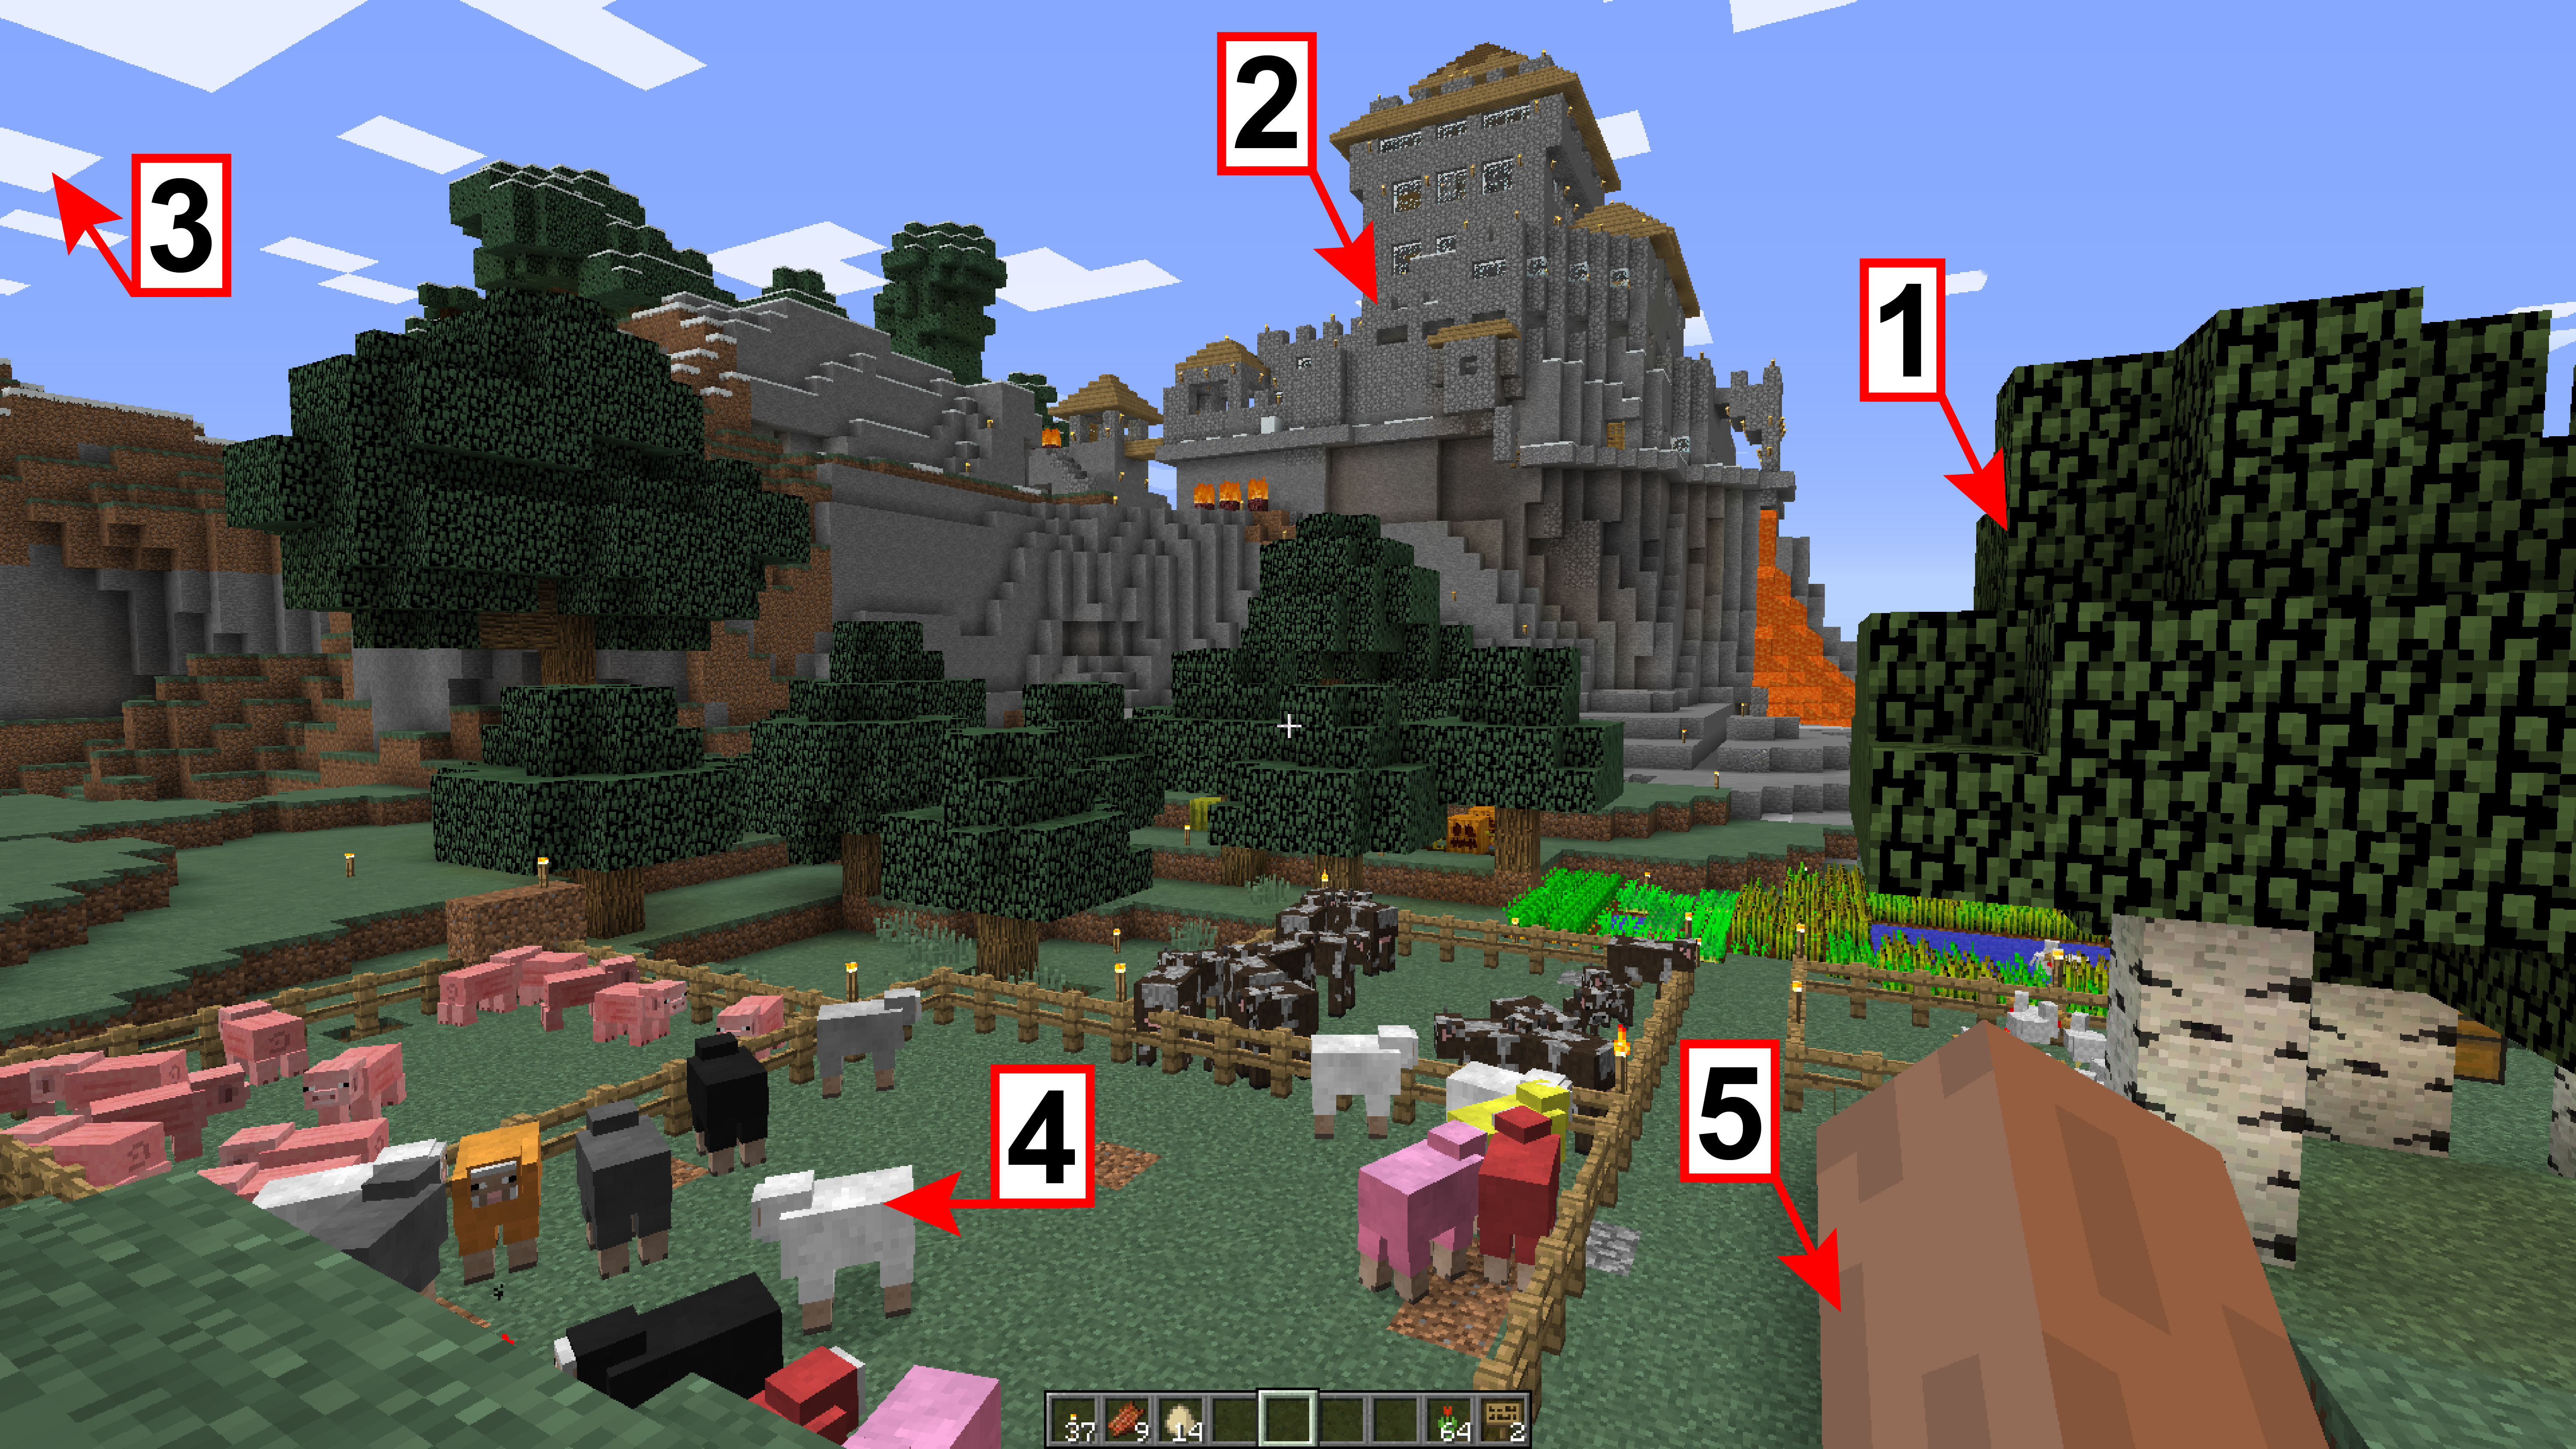
\includegraphics[ width=140mm]{../img/intro/mc}

\caption{Hra Minecraft - hrad na skále}
\label{fig:intro_mc}

\end{figure}

\FloatBarrier

Mezi dalšími hrami bychom mohli zmínit například \TE{}. Ta je o~něco mladší než \MC{}, ale je častým zdrojem diskusí, zda je lepší new \MC{}, nebo ne. Pravdou je, že obě hry mají svůj svět kompletně složený z~kostek (\TE{} je však 2D hra), ale každá si klade trochu jiné cíle. \TE{} je více orientovaná na příběh, obsahuje více \NPC{} i~bossů. Boss je v~herní terminologii významný nepřítel, obvykle je silnější než ostatní protivníci a~velmi často bývá v~závěrečných částech hry. Duel s~bossem pak obvykle od hráče vyžaduje zjištění jeho silných a~slabých stránek a~schémat jeho útoků \citep{intro_boss}. \MC{} je pak orientován spíše na stavění. (Porovnání Minecraft vs Terraria (facts) \citep{mc_te_comparsion} na Minecraftovém fóru.)


\subsection{Hry s~prvky realismu}

Mezi hry s~prvky realismu bychom mohli zařadit třeba hry \SE{} či \ME{}, využívají kombinaci herních bloků s~\textit{voxelovou} reprezentací světa. Obě hry jsou implementovány v~proprietárním enginu společnosti Keen Software House nazvaném \textit{VRAGE}\texttrademark{}. Voxelový terén je pak v~enginu za běhu hry procedurálně generován do polygonální reprezentace, kterou pak grafická karta standardním způsobem vykreslí na obrazovce (oficiální popis vlastností enginu \citep{vrage}). Během tohoto procedurálního vytváření je na třídimenzionální strukturu voxelů (které si můžeme představit jako bloky stejné velikosti) aplikován nějaký šum a~tím je možné ve hře vygenerovat prakticky neomezené množství různých objektů vycházejících z~jedné voxelové struktury. \uv{\textit{The “procedural asteroids” feature adds a~practically infinite number of asteroids to the game world}} \citep{rosa_blog}. Tímto způsobem pak hry dosáhují vyššího stupně realismu -- nespoléhají se pouze na předpřipravené 3D modely. 

Podívejme se na obrázek \ref{fig:intro_se} ze hry \SE{} (Zdroj: server Gamespot.com \citep{se_intro_img}). Na něm můžeme vidět převážně kamenný asteroid, a na něm je postavená vesmírná základna (obarvená zelenou barvou). K základně je přistavena větší vesmírná loď (modrobílá, v~levém horním rohu), hráč pak k~základně letí v~další, malé lodi (modrobílá uprostřed). Bližší pohled na planetku ukazuje, že její povrch není pravidelný. To je způsobeno právě algoritmickou aproximací voxelové reprezentace planetky. 

\begin{figure}[!ht]\centering
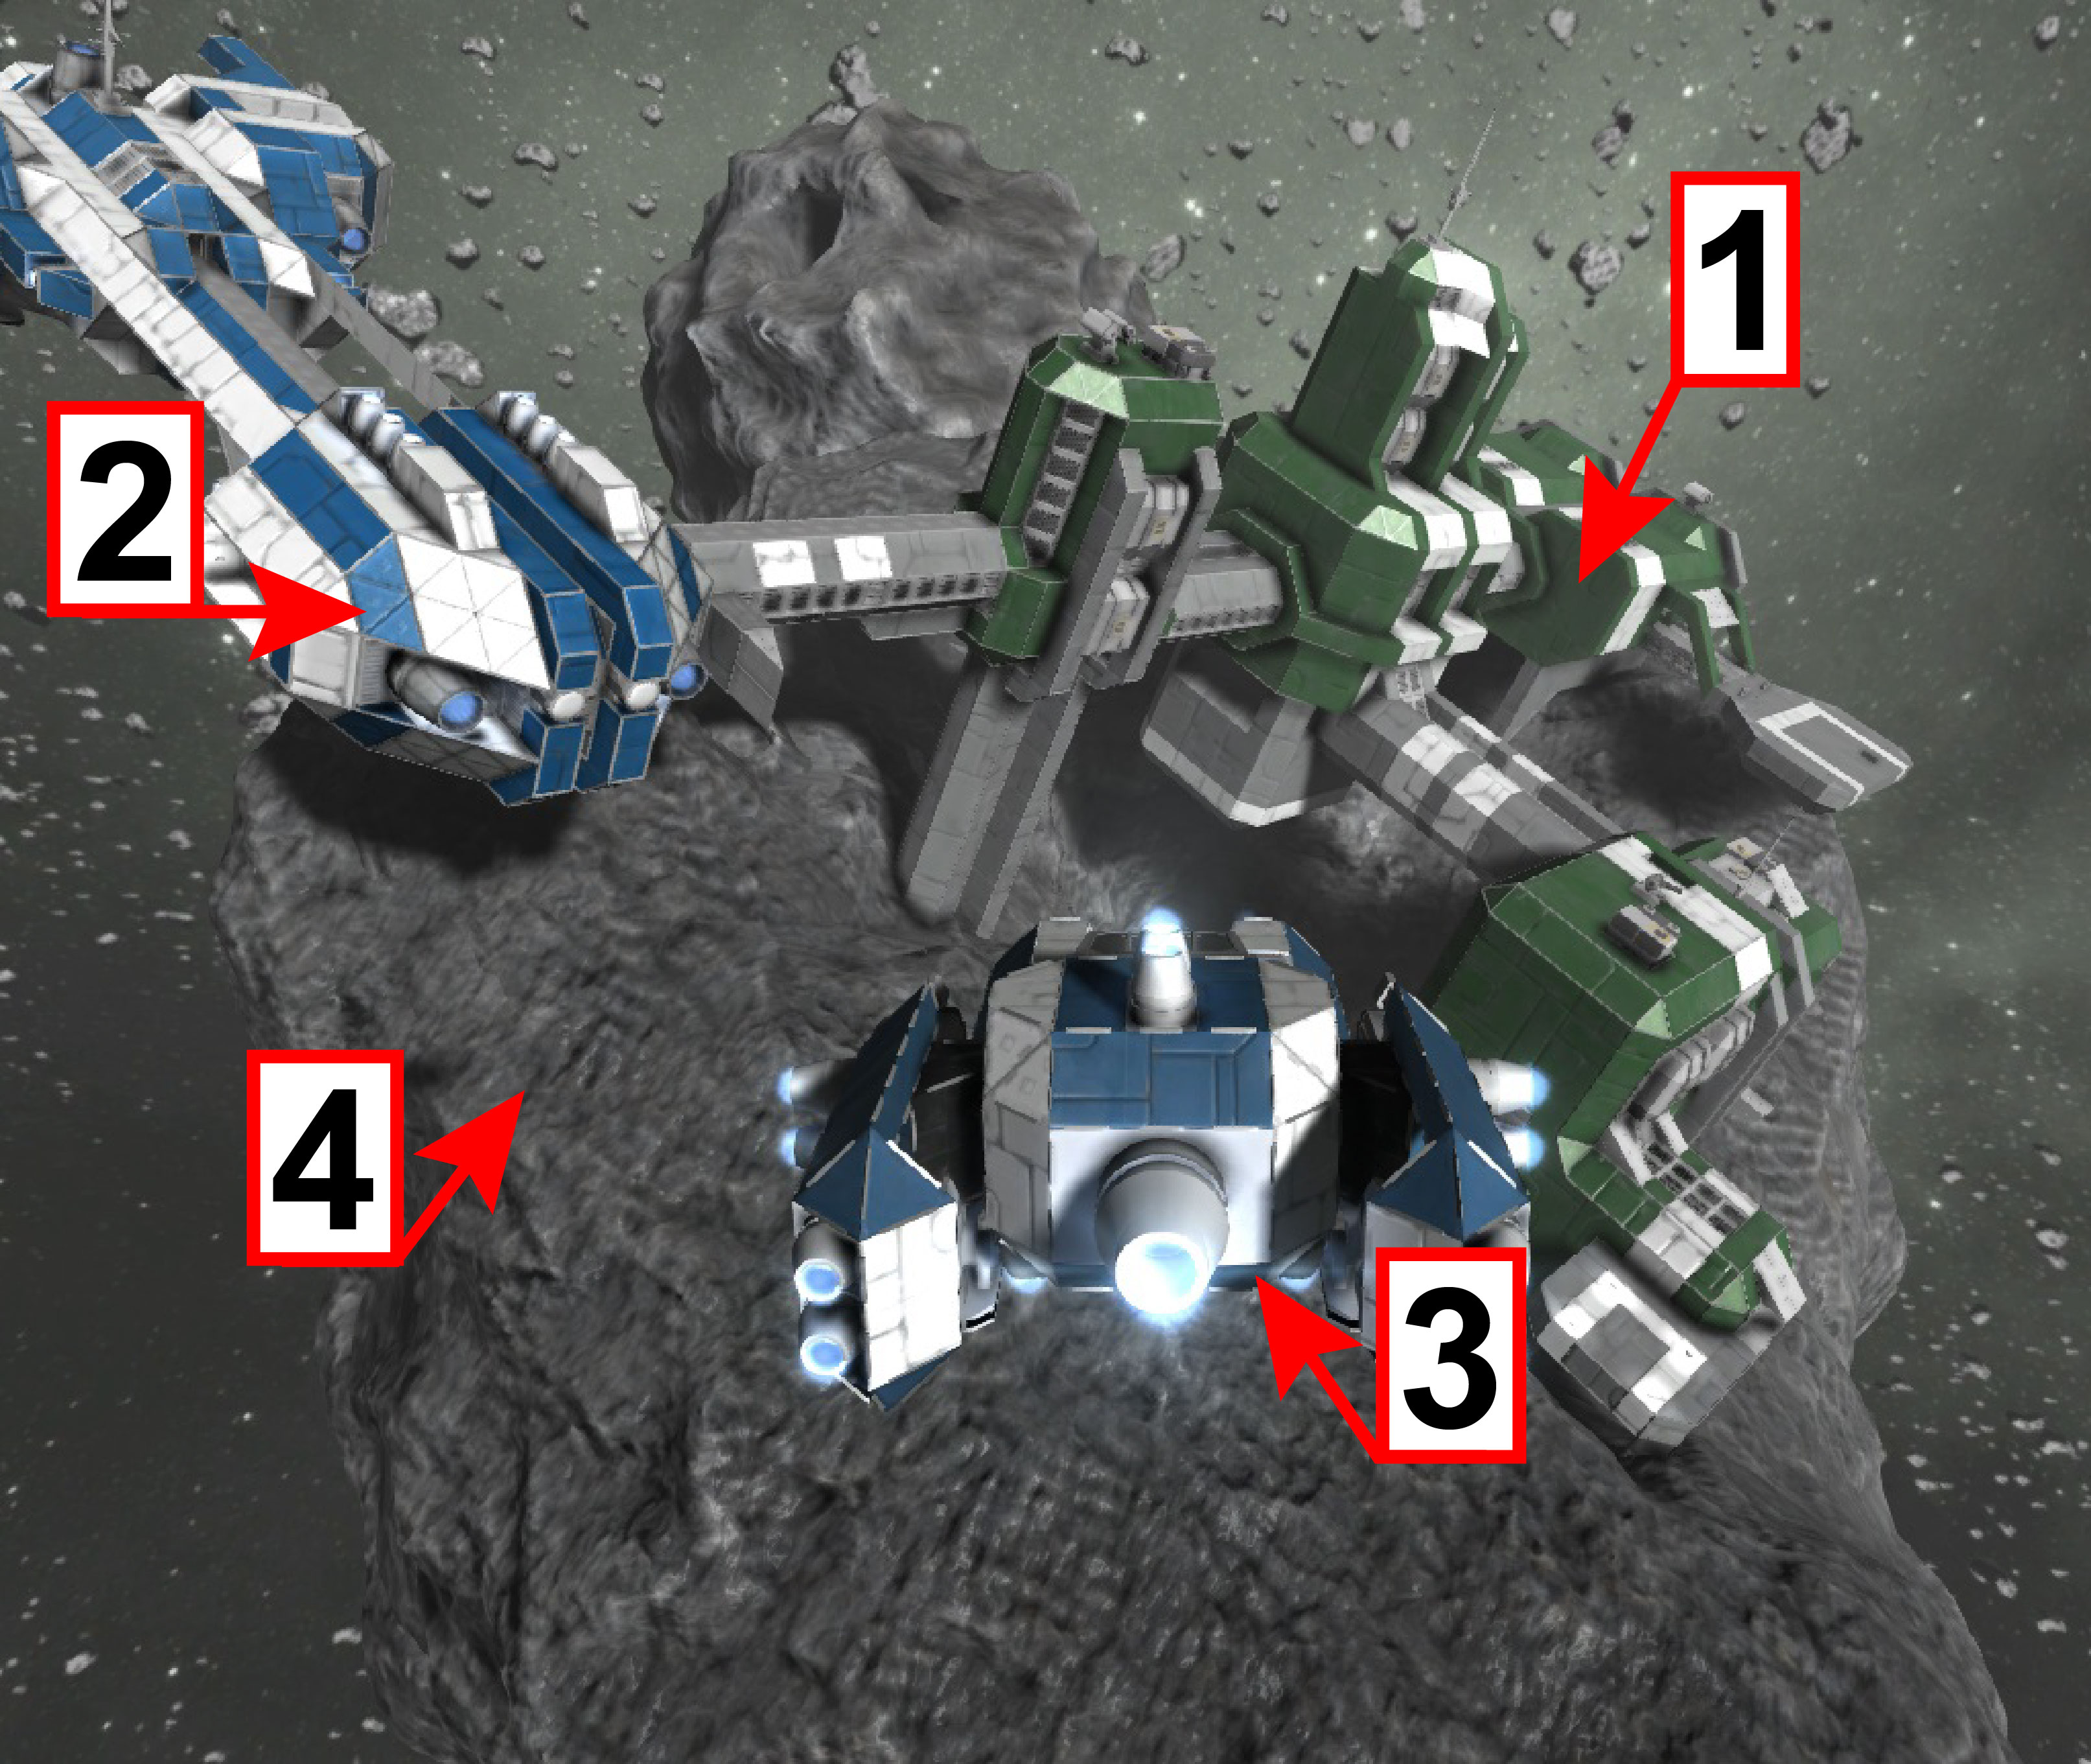
\includegraphics[ width=140mm]{../img/intro/se}

\caption{Hra Space Engineers - základna na asteroidu }
\label{fig:intro_se}

\end{figure}

\FloatBarrier

Samotná základna i~vesmírná plavidla (detailní pohled na jiné plavidlo je na obrázku \ref{fig:intro_se_ship}) jsou tvořeny bloky. Vizuální reprezentace bloku může být i~jiného tvaru než jen krychle -- to je možné vidět na obrázku \ref{fig:intro_se_blocks}). Barevně jsou zde zvýrazněny hranice bloků. Jak základny, tak vesmírné lodě (které jsou navíc oproti základnám pohyblivé) využívají tento systém. 

\SE{} umožňuje stavět pohyblivé stroje, které si hráč postaví z~herních bloků a~ty se pak chovají jako jedna entita. Stále je na ně však aplikována fyzika, takže je možné plavidlo poškodit, nebo dokonce zničit. Tento stupeň realismu od naší hry vyžadovat nebudeme. Budeme však chtít mít ve hře bloky, jejichž model není tvaru krychle. Stejně jako v \SE{} budeme chtít, aby bylo možné bloky rotovat v libovolném směru (u bloků, u kterých to bude dávat smysl).



\begin{figure}[!ht]\centering
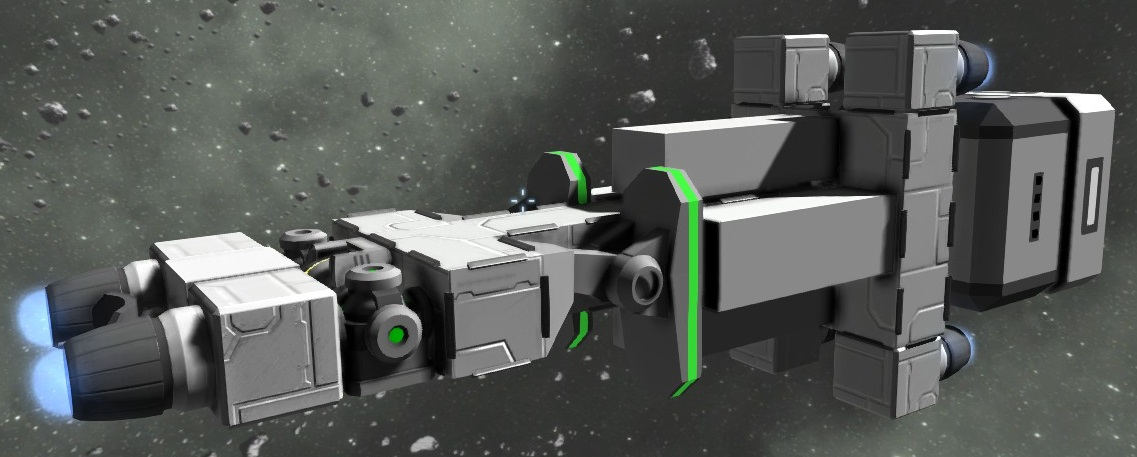
\includegraphics[ width=140mm]{../img/intro/se_ship}

\caption{Hra Space Engineers - vesmírná loď }
\label{fig:intro_se_ship}

\end{figure}

\begin{figure}[!ht]\centering
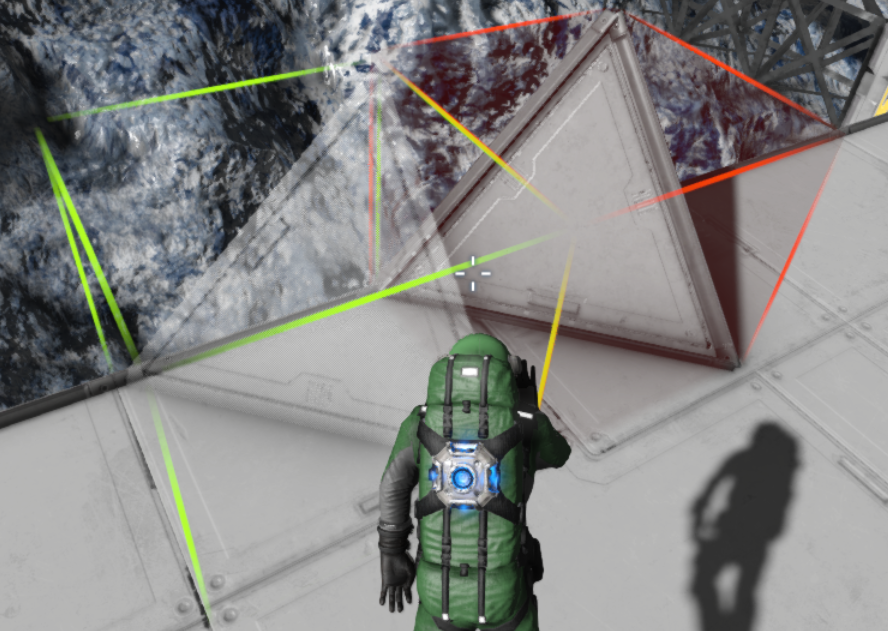
\includegraphics[ width=140mm]{../img/intro/se_blocks}

\caption{Hra Space Engineers - bloky }
\label{fig:intro_se_blocks}

\end{figure}

\FloatBarrier


\subsection{Hry s~maximálním důrazem na simulaci reality}

Do této sekce bychom měli zařadit například vesmírný simulátor \TM{}. // TODO popis, obrázek

bloky na stavění, ale třeba vozidla kompletní

\subsection{Ostatní - zařadit TODO }

Můžeme však nalézt i~další příklady her (// TODO \TM{}, \NI{}, \PN{}, \ARK{}, \NMS{}).



\section{Čemu se budeme věnovat}

Rádi bychom zachovali koncept použití herních bloků, který shledáváme jednoduchý na pochopení i~použití. Zaměříme se na rozšíření možnosti práce s~bloky tak, abychom uživateli nabídli, pokud možno, ještě lepší herní zážitek ze stavění vlastních výtvorů. V této práci se nebudeme nijak důkladně věnovat vizuální reprezentaci prostředí, protože ta pro nás v~tuto chvíli není podstatná. 

Změna v~přístupu k~herním blokům bude vyžadovat i~úpravy herního mechanismu s~tím souvisejícího -- hráčova inventáře. Všechny výše zmíněné hry nějakým způsobem nabízí hráči výběr bloků, které může do herního světa umístit. Naše změna by bohužel znamenala, že by se takový inventář postavitelných bloků velmi rychle stal nepřehledným a~proto musíme systém nabídky postavitelných bloků upravit pro naše potřeby.

\section{Herní bloky}



Obvykle je ve hře definován jeden základní rozměr bloku, který je neměnný. (\SE{} definuje více velikostí -- ty však nelze vzájemně kombinovat). To však může být problémem, pokud se hráč rozhodne postavit v~herním světě nějakou větší a~komplexnější strukturu podle reálné či fiktivní předlohy. Pro příklad uveďme některé výtvory ze hry \MC{} -- město Královo přístaviště z~knih Píseň ledu a~ohně od Geoge R. R. Martina, nebo hlavní město Gondoru Minas Tirith z~knih Pána prstenů od J. R. R. Tolkiena.

Autoři těchto výtvorů museli volit takové měřítko, aby byly výtvory dostatečně detailní, ale zároveň aby bylo možné výtvor postavit v~nějakém rozumném čase. Obecně můžeme říct, že čím větších detailů chtějí autoři ve hře \MC{} dosáhnout, tím větší musí celý výtvor být. To pak ale znamená, že celá stavba trvá déle, nebo je zapotřebí více spolupracujících hráčů. Hra \SE{} díky svému přístupu a~více bloků, které nejsou tvaru krychle, nabízí lepší možnosti staveb rozsáhlých objektů (představme si třeba Hvězdu smrti z~Hvězných válek), ale stále je potřeba volit nějakou rozumnou výslednou velikost.


\subsection{Náš návrh úpravy}
Chtěli bychom se v~této práci zabývat myšlenkou proměnlivé velikosti stavitelných bloků. Tím by hráči mohli rychleji stavět rozsáhlejší struktury a~přitom se věnovat i~drobným či estetickým detailům. Tento návrh však s~sebou nese několik problémů, které se v~této práci budeme snažit vyřešit.


\section{Inventář}
Dalším společným prvkem tohoto druhu her je inventář bloků, které může hráč umístit do herního světa. Hráč přes celé herní okno vidí \HUD{} (Head-Up Display \citep{hud_terminology}), ve kterém má zobrazenou kromě jiného nabídku bloků, které má na rychlé volbě, může je snadno zvolit a~daný blok umístit do herního světa. Navíc hry mohou definovat i~inventární skupiny bloků (\SE{}, \ME{}), mezi kterými hráč může přepínat a~tím rychle kompletně změnit sadu rychlé nabídky. Vidíme však limitaci v~tom, že hráč musí ručně spravovat tyto seznamy a~jednotlivé bloky (či nástroje) umisťovat do příslušných pozic.


\subsection{Náš návrh úpravy}
Rádi bychom navrhli jiný způsob správy těchto inventárních skupin, aby hráč jednou definoval, jaké prvky chce mít v~příslušných skupinách. Při vytvoření nového bloku či vytvoření jiné velikosti bloku by pak nemusel ručně přiřazovat nový blok do skupiny, ale tento blok by měl být automaticky zařazen a~nabídnut hráči.  




\section{Cíle práce}
Tato práce by měla naplnit následující cíle:
\begin{itemize}
	\item Navrhnout a~implementovat způsob řešení proměnlivé velikosti bloků
	\item Navrhnout a~implementovat automatizovanou správu inventáře
	\item Kvůli očekávaným nárokům na pochopení nových konceptů do hry implementovat výukový tutoriál (TODO má to být tady?)
	\item Získat a~zhodnotit zpětnou vazbu na výslednou hru
\end{itemize}

